\documentclass[border=10pt]{standalone}
\usepackage{tikz}
\usepackage{xcolor}
\definecolor{myred}{RGB}{195,20,45}

\begin{document}
	
	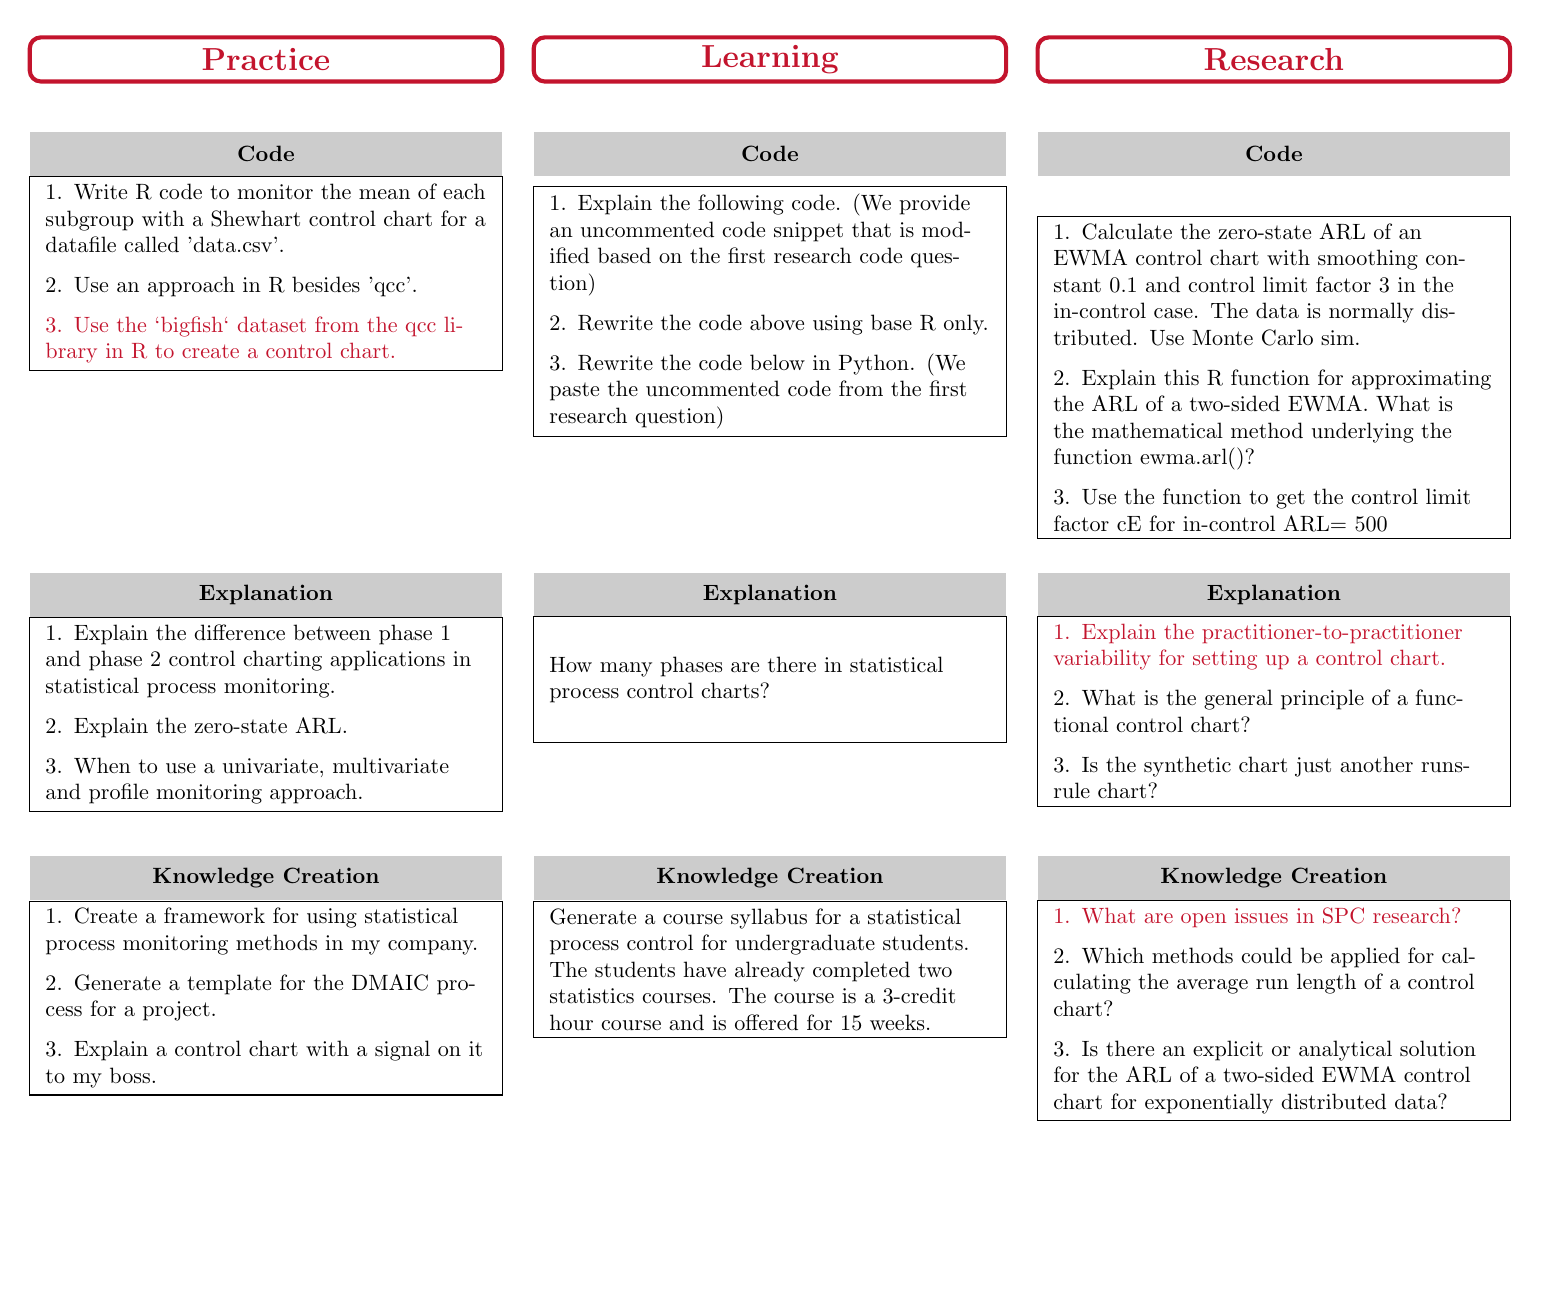
\begin{tikzpicture}[
		scale=0.8, every node/.style={scale=0.8}, % Adjust scale to fit content
		box/.style={rectangle, draw, minimum width=7.5cm, minimum height=2cm, align=left, text width=7cm},
		mainheader/.style={rectangle, draw=myred, minimum width=7.5cm, minimum height=0.7cm, fill=none, align=center, font=\bfseries\Large\color{myred}, text width=7cm, rounded corners, line width=1.5pt},
		header/.style={rectangle, draw=none, minimum width=7.5cm, minimum height=0.7cm, fill=black!20, align=center, font=\bfseries, text width=7cm}
		]
		
		% Define coordinate grid for positioning
		\draw[step=7cm,white,very thin,opacity=0.0] (-2,-19) grid (21,1);
		
		% Practice
		\node[mainheader](prac) at (1,0.5) {Practice};
		\node[header, below of=prac](prac-code-header)  at (1,0) {Code};
		\node[box, below of=prac-code-header](prac-code) at (1,-1.9) {
			1. Write R code to monitor the mean of each subgroup with a Shewhart control chart for a datafile called 'data.csv'. \\[6pt]
			2. Use an approach in R besides 'qcc'. \\[6pt]
			\textcolor{myred}{3.} \textcolor{myred}{Use the `bigfish` dataset from the qcc library in R to create a control chart.}
		};
		\node[header] at (1,-8) {Explanation};
		\node[box] at (1,-9.9) {
			1. Explain the difference between phase 1 and phase 2 control charting applications in statistical process monitoring. \\[6pt]
			2. Explain the zero-state ARL. \\[6pt]
			3. When to use a univariate, multivariate and profile monitoring approach.
		};
		\node[header] at (1,-12.5) {Knowledge Creation};
		\node[box] at (1,-14.4) {
			1. Create a framework for using statistical process monitoring methods in my company. \\[6pt]
			2. Generate a template for the DMAIC process for a project. \\[6pt]
			3. Explain a control chart with a signal on it to my boss.
		};
		
		% Learning
		\node[mainheader] (learn) at (9,0.5) {Learning};
		\node[header, below of=learn] (learn-code-header) at (9,0) {Code};
		\node[box=learn-code-header] (learn-code) at (9, -3.5){
			1. Explain the following code. (We provide an uncommented code snippet that is modified based on the first research code question) \\[6pt]
			2. Rewrite the code above using base R only. \\[6pt]
			3. Rewrite the code below in Python. (We paste the uncommented code from the first research question)
		};
		\node[header, below of=learn-code] (learn-exp-header) at (9, -7) {Explanation};
		\node[box=learn-exp-header] (learn-exp) at (9, -9.35) {
			How many phases are there in statistical process control charts?
		};
		\node[header, below of=learn-exp] (learn-kc-header) at (9, -11.5){Knowledge Creation};
		\node[box=learn-kc-header] (learn-kc) at (9, -13.95){
			Generate a course syllabus for a statistical process control for undergraduate students. The students have already completed two statistics courses. The course is a 3-credit hour course and is offered for 15 weeks.
		};
		
		% Research
		\node[mainheader] (res) at (17,0.5) {Research};
		\node[header, below of=res] (res-code-header) at (17,0) {Code};
		\node[box=res-code-header] (res-code) at (17,-4.55) {
			\textcolor{black}{1.} \textcolor{black}{Calculate the zero-state ARL of an EWMA control chart with smoothing constant 0.1 and control limit factor 3 in the in-control case. The data is normally distributed. Use Monte Carlo sim.} \\[6pt]
			\textcolor{black}{2.} \textcolor{black}{Explain this R function for approximating the ARL of a two-sided EWMA. What is the mathematical method underlying the function ewma.arl()?} \\[6pt]
			3. Use the function to get the control limit factor cE for in-control ARL=  500
		};
		\node[header, below of=res-code] (res-exp-header) at (17, -7)  {Explanation};
		\node[box=res-exp-header]  at (17, -9.85)(res-exp) {
			\textcolor{myred}{1. Explain the practitioner-to-practitioner variability for setting up a control chart.} \\[6pt]
			2. What is the general principle of a functional control chart? \\[6pt]
			3. Is the synthetic chart just another runs-rule chart?
		};
	\node[header, below of=res-exp] (res-kc-header) at (17, -11.5){Knowledge Creation};
	\node[box=res-kc-header] (res-kc) at (17, -14.6){
		\textcolor{myred}{1.} \textcolor{myred}{What are open issues in SPC research?} \\[6pt]
		2. Which methods could be applied for calculating the average run length of a control chart? \\[6pt]
		3. Is there an explicit or analytical solution for the ARL of a two-sided EWMA control chart for exponentially distributed data?
	};
	\end{tikzpicture}
	
\end{document}
